\documentclass[11pt]{article}
\usepackage[review]{acl}

\usepackage{times}
\usepackage{latexsym}
\usepackage[T1]{fontenc}
\usepackage[utf8]{inputenc}
\usepackage{microtype}

% inconsolata is recommended by the official ACL template for typewriter font
% aesthetics, but is not strictly necessary. Omitted here as it is not
% installed on the build system.
% \usepackage{inconsolata}

\usepackage{amsmath}
\usepackage{booktabs}
\usepackage{graphicx}
\usepackage{multirow}
\usepackage{subcaption}
\usepackage{pifont}
\usepackage{enumitem}

\usepackage{cleveref}

\graphicspath{{../figures/paper/}}

\setlength{\dbltextfloatsep}{6pt plus 2pt minus 2pt}
\setlength{\textfloatsep}{6pt plus 2pt minus 2pt}
\setlength{\floatsep}{6pt plus 2pt minus 2pt}
\setlength{\intextsep}{4pt plus 2pt minus 2pt}
\setlength{\abovecaptionskip}{4pt}
\setlength{\belowcaptionskip}{0pt}

\title{Temporal Score Incomparability in LLM Benchmarks:\\A Large-Scale Psychometric Audit of 5,227 Models}

\begin{document}

\maketitle

\begin{abstract}
Large language model (LLM) benchmark scores are routinely compared across model generations, yet whether individual items measure the same construct over time is rarely tested. We apply differential item functioning (DIF) analysis from educational measurement to the METABENCH response matrix (5,227 models on MMLU, replicated across six benchmarks), validated through semi-synthetic injection with a cross-subject matching guarantee. Between 2023 and 2024 model cohorts, 18--31\% of items exhibit large temporal DIF, 45--95$\times$ above random baselines, while aggregate rankings remain near-perfect ($\rho \geq 0.994$). DIF flags are near-independent of web-overlap contamination labels ($\phi = 0.012$), indicating that global exposure and differential functioning are complementary diagnostic dimensions. Base and instruct models exhibit opposite DIF directions, confirming structured capability shifts beyond contamination. We propose a three-step Monitor/Triage/Correct audit protocol with empirically grounded thresholds for benchmark maintainers. LLM benchmarks need psychometric monitoring, not just score reporting\footnote{Code and data are available at \url{https://anonymous.4open.science/r/irt_equated_bench_regen-2431/}.}.
\end{abstract}

\section{Introduction}
\label{sec:introduction}

\looseness=-1
When we say ``Model B outperforms Model A on MMLU,'' we assume that every test item measures the same construct for both models. In educational testing, this property, \emph{measurement invariance}~\citep{meredith1993invariance}, is routinely verified before scores are compared across groups; in LLM evaluation, it has never been tested at scale. We test it here, applying Mantel-Haenszel differential item functioning (DIF) analysis~\citep{holland1988mh} with Educational Testing Service (ETS) severity classification to the METABENCH response matrix~\citep{kipnis2024metabench} (5,227 models $\times$ 12,508 MMLU~\citep{hendrycks2021mmlu} items). The result is sobering: 31\% of items receive ETS Category~C classification ($|\Delta_{\mathrm{MH}}| \geq 1.5$, $p < 0.05$) between 2023 and 2024 model cohorts, compared to 0.62\% under random-split controls, and the finding replicates across all six METABENCH benchmarks (17.9--31.3\%).

\begin{figure*}[t]
\centering
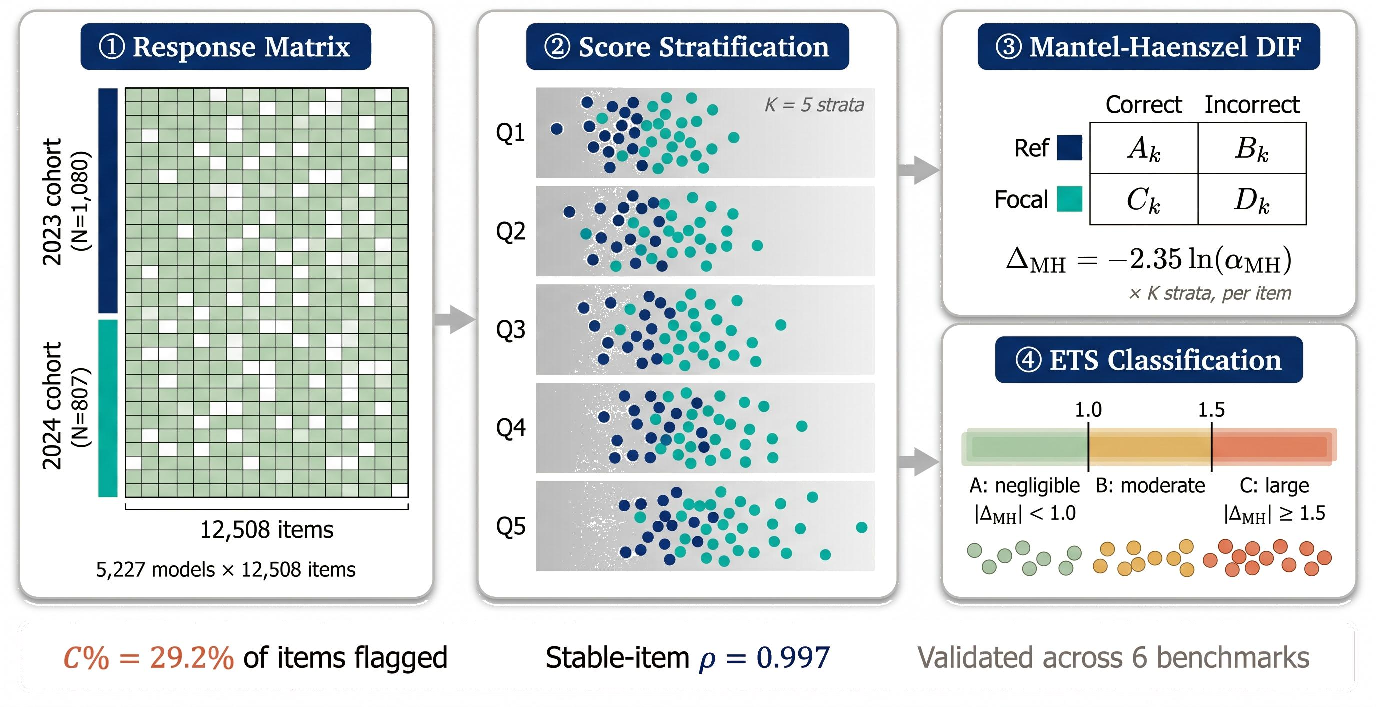
\includegraphics[width=\textwidth]{fig_0_pipeline.pdf}
\caption{Four-stage psychometric auditing pipeline. \textbf{\ding{192}} A binary response matrix records model correctness across benchmark items, with models split into temporal cohorts (2023 reference vs.\ 2024 focal). \textbf{\ding{193}} Models are stratified into $K{=}5$ score quintiles. \textbf{\ding{194}} Per-item Mantel-Haenszel DIF tests compute $\Delta_{\mathrm{MH}}$ across strata. \textbf{\ding{195}} ETS classification assigns severity labels (A/B/C). Result: 31.3\% of items flagged as C (29.2\% after design-effect (DEFF) correction), yet stable-item $\rho = 0.997$, replicated across six benchmarks.}
\label{fig:pipeline}
\end{figure*}

\looseness=-1
This instability is not what it appears. Aggregate rankings are near-perfect ($\rho \approx 0.997$): even after all unstable items are removed, the leaderboard barely changes. But individual items have shifted in structured ways: some became easier for newer models independent of overall ability, others harder, and these differential effects can shift individual models by ${\pm}561$ rank positions at the 99th percentile (\Cref{app:rank_reversal}). Instability does not threaten validity; it reveals which capability dimensions shift across model generations. Base and instruct models exhibit opposite DIF directions ($\chi^2 = 562.7$), which confirms structured capability changes, not noise.

\looseness=-1
This diagnostic signal is distinct from what existing benchmark integrity methods target. Contamination detection asks whether items appear in training corpora, probing \emph{global exposure}~\citep{shi2024mink,dekoninck2024constat,liang2026dvd,tao2026selfcritique}, validated against web-overlap labels~\citep{li2024contamination}. Measurement invariance asks whether items \emph{function equivalently} across model cohorts (\Cref{fig:global_vs_differential}). We find these two signals are near-independent (Jaccard~$= 0.206$, $\phi = 0.012$): complementary diagnostic dimensions, not competing ones. Any item-level detector validated solely against web-overlap labels is blind to differential functioning.

\begin{figure*}[t]
\centering
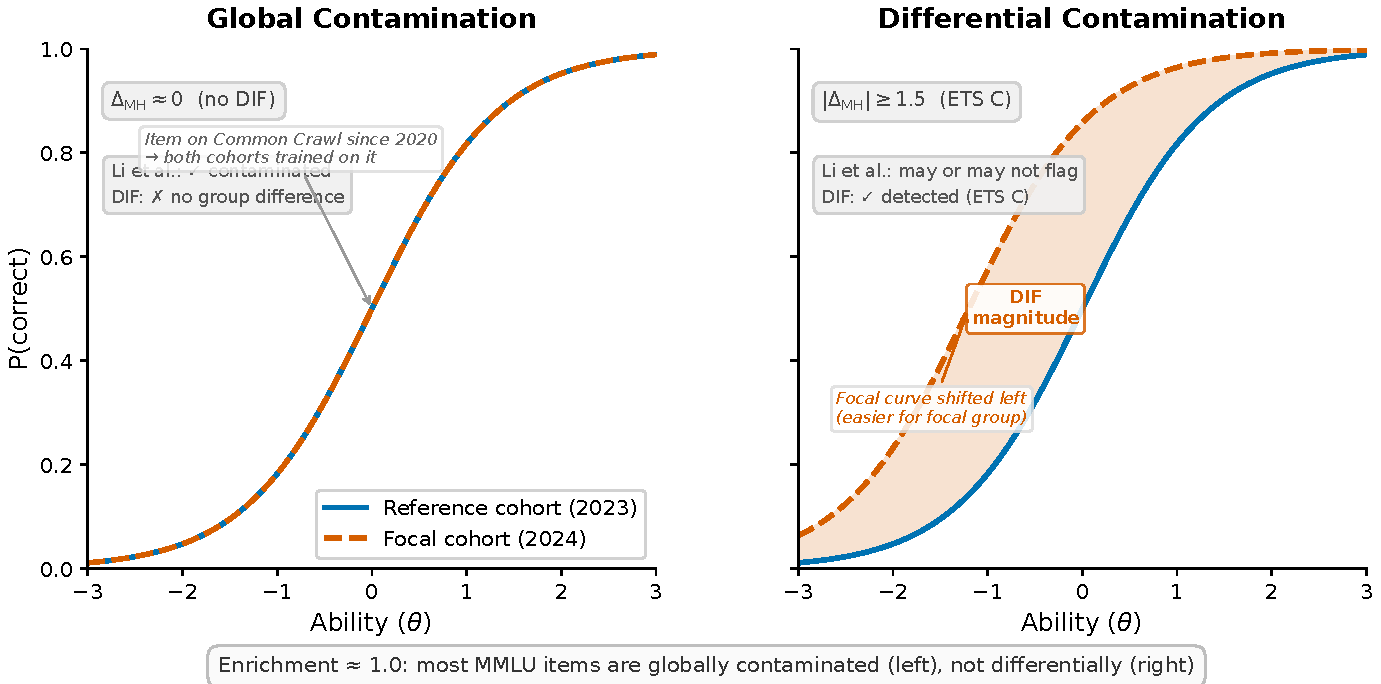
\includegraphics[width=\textwidth]{fig_1_global_vs_differential.pdf}
\caption{Global vs.\ differential contamination via Item Characteristic Curves (ICCs). \textbf{Left}: global contamination produces no DIF; both cohorts encounter the item, and their ICCs overlap. \textbf{Right}: differential contamination produces DIF; the focal cohort's ICC shifts due to disproportionate exposure. The enrichment ratio of $\approx 1.0$ between DIF flags and web-overlap labels is expected because most items fall into the left category.}
\label{fig:global_vs_differential}
\end{figure*}

\looseness=-1
To our knowledge, this is the largest-scale DIF analysis on LLM benchmarks, complementary to concurrent work on anchor-item calibration~\citep{habba2026growingpains} and motivated by the fragility of existing detectors under post-training perturbation~\citep{wang2026fragility}. We make three contributions:
\begin{enumerate}[nosep,leftmargin=*,topsep=2pt]
\item \textbf{Temporal DIF at scale}: 31.3\% of MMLU items exhibit large temporal DIF (17.9--31.3\% across six benchmarks; 29.2\% after non-independence correction), near-independent of web-overlap labels (Jaccard $= 0.206$); base-vs-instruct stratification reveals opposite patterns ($\chi^2 = 562.7$), consistent with structured capability shifts rather than uniform exposure (\Cref{sec:temporal,sec:groundtruth,sec:gsm8k,sec:disc_temporal}).
\item \textbf{Semi-synthetic validation with $\Delta\mathrm{FPR} = 0$ guarantee}: cross-subject matching eliminates false-positive inflation under single-subject contamination ($k \leq 5$), portable across benchmarks (\Cref{sec:semisynthetic}).
\item \textbf{DIF as diagnostic lens with actionable audit protocol}: unstable items carry disproportionate cross-cohort signal ($z = -8$ to $-49\sigma$) yet are the least ranking-disruptive under non-random removal, which confirms that DIF isolates differential functioning rather than generally informative items; we propose a Monitor/Triage/Correct protocol for benchmark maintainers (\Cref{sec:disc_protocol}).
\end{enumerate}

\section{Related Work}
\label{sec:related_work}

\paragraph{DIF Methodology and Measurement Invariance.}
The Mantel-Haenszel procedure for DIF detection was introduced by \citet{holland1988mh} and remains the most widely used method in educational testing due to its simplicity and well-characterized statistical properties \citep{clauser1998dif}. Alternative approaches include logistic regression DIF \citep{swaminathan1990logistic}, SIBTEST \citep{shealy1993sibtest}, Lord's $\chi^2$ test \citep{lord1980irt}, and the Raju area method \citep{raju1988area}; \citet{millsap1993dif}, \citet{zumbo1999handbook}, and \citet{penfield2007dif} provide comprehensive reviews. DIF analysis is a specific instance of measurement invariance testing \citep{meredith1993invariance, vandenberg2000invariance, millsap2011invariance}, which examines whether a measurement instrument functions equivalently across populations. MIMIC models offer a latent-variable approach to the same problem \citep{muthen1985mimic, woods2009mimic}, and \citet{teresi2007dif} reviews DIF methods across applied domains. Cross-subject matching---computing the stratification variable from domains other than the one being tested---adapts purified subtest matching from the DIF literature \citep{nandakumar1993dif,donoghue1993mh} to a new challenge: contamination control at scale, where the matching variable itself may be compromised by the phenomenon under test. We retain the standard MH statistic and develop LLM-specific adaptations around it: cross-subject matching for contamination control (with a constructive $\Delta\mathrm{FPR} = 0$ guarantee), DEFF correction for non-independence, and semi-synthetic validation absent ground-truth labels. The 5,227-examinee scale exceeds typical DIF applications~\citep{belzak2020smallsample}. The impact-versus-DIF confound is addressed through matched-ability quintile analysis, IRT $\theta$-conditioning (as sensitivity check), and a random-split control (\Cref{sec:temporal}).

\paragraph{IRT in LLM Evaluation.}
IRT adoption in LLM evaluation has accelerated: \citet{lalor2019irt} introduced IRT to NLP, \citet{vania2021irt} assessed test set discriminability, and \citet{rodriguez2021evaluation} demonstrated that not all evaluation examples are equally informative. Recent extensions include PSN-IRT \citep{zhou2026psnirt} for benchmark quality at scale, TinyBenchmarks \citep{maiapolo2024tinybenchmarks} for IRT-based item selection, scalability coefficients for detecting bad benchmark items \citep{hardy2026scalability}, IRT-based evaluation quality~\citep{kraus2024irt}, ATLAS \citep{li2025atlas} for computerized adaptive testing of LLMs, JE-IRT \citep{yao2025jeirt} for geometric ability embedding, continuous-score adaptive evaluation~\citep{balkir2026confident}, and competency-focused IRT evaluation in medical domains \citep{luo2025medirt}. The closest concurrent work is Growing Pains \citep{habba2026growingpains}, which uses IRT calibration to establish anchor items for cross-temporal score equating via fixed-parameter calibration \citep[FPC;][]{kim2019fpc}. While Growing Pains uses parametric IRT (2PL/3PL fixed-parameter calibration), MH-DIF is nonparametric and robust to model misspecification---an advantage given poor 2PL fit for MMLU (RMSEA $> 0.08$; \Cref{app:power_sensitivity}). Growing Pains prescribes how to equate scores after instability is detected; our work diagnoses \emph{which} items exhibit instability and quantifies severity via ETS classification, providing pre-screened anchor candidates for downstream equating. Their anchor-item selection can directly consume our stable-item set as pre-screened candidates; our finding that 31\% of items exhibit temporal DIF identifies which items should \emph{not} serve as anchors. To our knowledge, no prior work applies DIF to benchmark temporal comparability---contamination detection and psychometric evaluation optimization have developed as separate threads.

\paragraph{Contamination Detection.}
A growing family of methods detects benchmark contamination through model behavior or training data analysis. Membership inference approaches estimate whether a model has seen specific items during training: Min-K\% \citep{shi2024mink} and Min-K\%++ \citep{zhang2024minkpp} use token-level log-likelihood statistics, while Time Travel \citep{golchin2024timetravel} probes models with temporal cues and \citet{oren2024proving} prove contamination through exchangeability tests. Performance-based detectors identify contamination through statistical anomalies \citep{dekoninck2024constat,liang2026dvd,tao2026selfcritique,deng2024investigating} in-context learning effects~\citep{zawalski2026codec}, or inference-time decontamination~\citep{chai2026benchmarksleak}. \citet{balloccu2024leak} provide a broader taxonomy of leakage detection strategies. These methods share a common validation practice: they verify detection accuracy against web-overlap or n-gram labels \citep{li2024contamination} that classify items based on verbatim matches in publicly accessible corpora. Such labels measure \emph{global exposure} (whether an item exists in training data) rather than \emph{differential item functioning} (whether an item behaves differently across model cohorts). This global-vs-differential distinction motivates our comparison with web-overlap labels (\Cref{sec:groundtruth}). Work on LLM memorization \citep{carlini2022quantifying, tirumala2022memorization} establishes that memorization depends on data frequency and model scale, reinforcing the distinction between global exposure and differential behavior. \citet{wang2026fragility} show that existing contamination detectors are fragile under reinforcement learning, further motivating behavioral approaches grounded in psychometric theory.

\paragraph{Benchmark Quality and Design.}
Meta-evaluation of static benchmark quality~\citep{zhu2026bhi,qian2026benchmark2} assesses quality at a single snapshot; our temporal DIF analysis diagnoses \emph{when} measurement properties shift. MMLU-CF~\citep{zhao2025mmlucf} reconstructs contamination-free items and MMLU-Pro~\citep{wang2024mmlupro} extends item difficulty; DIF monitoring identifies which existing items remain measurement-invariant without replacement. \citet{maeda2025difllm} use LLMs to predict DIF in human assessments---the reverse direction; we apply DIF to LLM benchmarks with models as examinees. Dynamic benchmarks~\citep{kiela2021dynabench,li2024latesteval,white2025livebench} and self-evolving frameworks~\citep{ying2024automating,xu2025benchmark} mitigate contamination by construction but lack psychometric equating. Broader surveys~\citep{chang2024survey,burnell2023rethink,alzahrani2024benchmarks} identify benchmark saturation as a systemic challenge that DIF analysis directly addresses.

\section{Method}
\label{sec:method}

We adopt Differential Item Functioning (DIF) analysis from educational measurement to assess whether individual benchmark items behave consistently across groups of LLMs. The procedure requires only a binary response matrix and group labels, with no access to model internals or training data. Below we define the data, the statistical test, the cohort designs, a semi-synthetic validation framework, diagnostic checks, and statistical controls.

\subsection{Data}
\label{sec:data}

The primary dataset is the METABENCH response matrix~\citep{kipnis2024metabench}, which records binary outcomes (1~=~correct, 0~=~incorrect) for 5,227 models evaluated on 12,508 MMLU items~\citep{hendrycks2021mmlu}. Models span release dates from 2023 to 2024, drawn from the Open LLM Leaderboard. MMLU covers 57 subjects grouped into five broad domains (STEM, Humanities, Social Sciences, Other, and a mixed category). We supplement the response matrix with the web-overlap contamination labels of \citet{li2024contamination}, which classify 9,229 of 12,508 items (73.8\% coverage) as ``contaminated'' or ``clean'' based on verbatim matches in publicly accessible web corpora. These labels serve as an external reference for evaluating the relationship between DIF flags and existing contamination indicators.

\subsection{Mantel-Haenszel DIF and ETS Classification}
\label{sec:mhdif}

In educational testing, Differential Item Functioning (DIF) occurs when an item's statistical relationship to the latent trait $\theta$ differs between two groups after conditioning on ability level. An item with DIF is not merely harder for one group; it functions differently relative to what the group's overall ability would predict. The standard terminology refers to test-takers as ``examinees'' and questions as ``items.'' In our setting, examinees are LLMs and items are benchmark questions.

The Mantel-Haenszel (MH) procedure~\citep{holland1988mh} detects DIF by stratifying examinees into $K$ score bins based on total score (a proxy for $\theta$), where $K$ equals the number of distinct total scores observed in the combined sample, and computing a common odds ratio across strata. Within each stratum $k$, the responses of the reference group and the focal group form a $2 \times 2$ contingency table:

\begin{equation}
\label{eq:mh}
\alpha_{\mathrm{MH}} = \frac{\displaystyle\sum_{k=1}^{K} A_k D_k \,/\, T_k}{\displaystyle\sum_{k=1}^{K} B_k C_k \,/\, T_k}\,,
\end{equation}

\noindent where $A_k$ and $B_k$ are the number of correct and incorrect responses in the reference group for stratum $k$, $C_k$ and $D_k$ are the corresponding counts for the focal group, and $T_k$ is the total number of examinees in stratum $k$. Under the null hypothesis of no DIF, $\alpha_{\mathrm{MH}} = 1$. The log odds ratio is converted to the ETS delta scale:

\begin{equation}
\label{eq:delta}
\Delta_{\mathrm{MH}} = -2.35 \ln(\alpha_{\mathrm{MH}})\,.
\end{equation}

The Educational Testing Service (ETS) classifies DIF severity into three categories based on $|\Delta_{\mathrm{MH}}|$. Category~A (negligible) requires $|\Delta_{\mathrm{MH}}| < 1.0$. Category~C (large) requires both $|\Delta_{\mathrm{MH}}| \geq 1.5$ and statistical significance at $p < 0.05$ from the MH chi-squared test. Category~B (moderate) includes all remaining items: those with $1.0 \leq |\Delta_{\mathrm{MH}}| < 1.5$, or $|\Delta_{\mathrm{MH}}| \geq 1.5$ without statistical significance. The dual threshold in ETS~C (effect size \emph{and} significance) guards against flagging items that show large but unreliable effect sizes. Throughout this paper, we report the percentage of items classified as ETS~C, denoted C\%.

The choice of matching variable (the total score used for stratification) affects both validity and interpretation. We distinguish three matching strategies: (1)~\emph{standard matching} uses the within-benchmark total score on all items of the same benchmark; (2)~\emph{cross-subject matching} uses the total score on all subjects \emph{other than} the one containing the item under test, preventing the matching variable from absorbing injected contamination signals (\Cref{sec:injection}); and (3)~\emph{external matching} uses the total score on a different benchmark entirely (e.g., MMLU total score as the matching variable when testing DIF on GSM8K items), providing an independent ability proxy uncontaminated by the target benchmark. Cross-subject and external matching both address matching variable contamination but at different granularities: cross-subject operates within a multi-domain benchmark, while external operates across benchmarks.

\subsection{Cohort Designs}
\label{sec:cohorts}

DIF requires defining a reference group and a focal group. We construct five cohort comparisons, each designed to isolate a different source of variation.

\paragraph{Temporal.} The reference group consists of models released in 2023 ($N = 1{,}080$) and the focal group consists of models released in 2024 ($N = 807$). This is the primary comparison for detecting items whose functioning changed across model generations.

\paragraph{Ability-quintile.} Models within the same temporal window are divided by total score into quintiles. The focal group contains the lowest-scoring models (Q1--Q2) and the reference group contains the highest-scoring models (Q4--Q5). This comparison tests whether ability differences alone produce DIF, without temporal confounds.

\paragraph{Within-family.} Llama-2 models ($N = 161$) serve as the reference group and Llama-3 models ($N = 308$) as the focal group. This comparison isolates generational changes within a single model family.

\paragraph{Within-subject.} DIF is computed separately for each of the 57 MMLU subjects, with the matching variable (total score) restricted to items within the same subject. This design tests whether instability concentrates in specific knowledge domains.

\paragraph{Random split.} The 2023 cohort is divided into two equal random halves ($N = 540$ each). This serves as a sanity check: no systematic DIF should appear between two random subsets of the same population (expected C\% $\approx 0$).

\subsection{Semi-Synthetic Injection Framework}
\label{sec:injection}

To evaluate whether MH-DIF can detect differential contamination when it is present, we construct a semi-synthetic framework with controlled ground truth.

\paragraph{Procedure.} From items classified as ETS~A in the uninjected data (negligible DIF), we select 20\% uniformly at random as the ``contaminated'' set. For each contaminated item, we flip incorrect responses to correct in the focal group at exploitation rate $p \in \{0.0, 0.3, 0.5, 0.7, 1.0\}$. We then run MH-DIF on the modified response matrix and measure detection performance. We report $\Delta\mathrm{TPR} = \mathrm{TPR}(\text{injected}) - \mathrm{TPR}(\text{baseline})$ and $\Delta\mathrm{FPR} = \mathrm{FPR}(\text{injected}) - \mathrm{FPR}(\text{baseline})$, where TPR is the true positive rate on injected items and FPR is the false positive rate on uninjected items. Each injection level is repeated across 5 random seeds for uncertainty estimation.

\paragraph{Cross-subject matching.} The choice of matching variable is critical for valid semi-synthetic evaluation. When contamination is injected into items within subject $X$, the total score on subject $X$ absorbs part of the injection signal. Using this contaminated total score as the MH matching variable violates the conditional independence assumption and inflates FPR. Cross-subject matching resolves this problem by computing the matching variable from all subjects \emph{other than} the one being tested. Under this protocol, $\Delta\mathrm{FPR} = 0.000$ across all five MMLU domains, while detection power is preserved ($\Delta\mathrm{TPR} > 0.3$ at $p = 0.5$ for four of five subjects). We adopt cross-subject matching as the standard protocol for all semi-synthetic analyses.

\subsection{Diagnostics}
\label{sec:diagnostics}

Three diagnostic procedures complement the primary DIF analysis.

\paragraph{Local independence (Yen's Q3).} The MH procedure assumes that item responses are conditionally independent given $\theta$. Yen's Q3 statistic measures residual correlations between item pairs after conditioning on the latent trait. We compute Q3 for all within-subject and cross-subject item pairs, with $|Q3| > 0.20$ as the threshold for local dependence. Elevated within-subject dependence would indicate that items within the same subject share variance beyond what $\theta$ captures, which could inflate within-subject DIF rates.

\paragraph{Domain-specificity.} We test whether temporal DIF concentrates in domains where models improved most. At the ecological level, we compute Spearman $\rho$ between subject-level C\% and subject-level accuracy improvement from 2023 to 2024. At the item level, logistic regression predicts item-level DIF~C classification from domain-level accuracy change, with and without item property controls (difficulty, discrimination). This decomposition quantifies how much of the observed instability is attributable to aggregate domain-level gains versus item-specific behavioral change.

\paragraph{Instability decomposition.} When domain accuracy improvement is included alongside item-level controls, we compute the counterfactual C\% that would remain after removing domain-level effects. The gap between observed and counterfactual C\% measures the contribution of domain-level improvement to the total instability.

\subsection{Statistical Considerations}
\label{sec:statistical}

\paragraph{Multiple testing.} The ETS~C classification imposes a dual threshold (effect size $|\Delta_{\mathrm{MH}}| \geq 1.5$ and significance $p < 0.05$), which provides implicit control over false positives. As a robustness check, we apply Benjamini-Hochberg FDR correction at $q = 0.05$. The random-split sanity check provides an empirical estimate of the false positive rate under the null hypothesis.

\paragraph{Threshold sensitivity.} We report results across a range of DIF thresholds ($|\Delta_{\mathrm{MH}}| \in \{1.0, 1.5, 2.0, 2.5\}$) to verify that qualitative conclusions do not depend on the specific ETS~C cutoff. The standard threshold of $|\Delta_{\mathrm{MH}}| \geq 1.5$ corresponds to the ETS~C definition used throughout the paper.

\paragraph{Architecture heterogeneity.} The METABENCH MMLU population consists of 99.98\% decoder-only models (5,226 of 5,227). This near-complete architectural homogeneity eliminates architecture as a confound for DIF analysis. We verify this by excluding the single encoder-decoder model and confirming identical results.

\section{Experiments}
\label{sec:experiments}

We apply MH-DIF to the METABENCH dataset~\citep{kipnis2024metabench}, which provides sparse response matrices for 5,227 models evaluated on 12,508 MMLU items~\citep{hendrycks2021mmlu}. All temporal analyses define reference and focal cohorts by model release date (2023 vs.\ 2024). We validate detection power through simulation, characterize temporal instability across multiple cohort designs, evaluate the relationship between DIF flags and existing contamination labels, and assess downstream consequences for benchmark rankings. Replication on GSM8K with cross-benchmark contamination validation appears in \Cref{sec:gsm8k}.

\subsection{Validation: DIF Detection Power}
\label{sec:validation}

To confirm that MH-DIF detects differential item functioning at the sample sizes available in METABENCH, we conduct a power analysis using empirical MMLU IRT parameters. We simulate item response matrices where a controlled subset of items has injected DIF of varying magnitude ($|\Delta_{\mathrm{MH}}| \geq 1.4$) and evaluate ETS~C classification across sample sizes $N \in \{40, 80, 160, 320\}$ per cohort. At $N \geq 80$, ETS~C achieves true positive rates of 0.68--0.80 with false positive rates of 0.036--0.042 and AUC of 0.93--0.94. The temporal cohort sizes in our analysis ($N_{\mathrm{ref}} = 1{,}080$, $N_{\mathrm{focal}} = 807$) far exceed this threshold, and statistical power is not a limiting factor for the results reported below. Full simulation results with confidence intervals appear in Appendix~Table~A1.

\subsection{Temporal Comparability: 31\% Item Instability}
\label{sec:temporal}

The central finding of this paper is that a substantial fraction of MMLU items behave differently across model generations. Comparing models released in 2023 ($N = 1{,}080$) against models released in 2024 ($N = 807$), 31.3\% of items receive ETS~C classification ($|\Delta_{\mathrm{MH}}| \geq 1.5$). Applying Benjamini-Hochberg FDR correction at $q = 0.05$ reduces this from 31.32\% to 31.30\%, removing only 3 items. The minimal impact of FDR correction reflects the fact that the ETS classification system imposes a dual threshold on both effect size and statistical significance, which already provides implicit multiple-testing protection. In absolute terms, nearly one in three MMLU items exhibits a large shift in its statistical relationship to overall model ability between the two cohort periods.

Three control conditions establish that this instability reflects genuine temporal change rather than methodological artifacts. A random split of the 2023 cohort into two equal halves produces only 0.18\% ETS~C items, confirming that sampling noise alone does not generate large-scale DIF. An ability-quintile comparison (lowest-scoring vs.\ highest-scoring models within the same temporal cohort) yields 2.9\% ETS~C items, indicating that ability differences alone are insufficient to produce the observed instability. A within-family comparison of Llama-2 ($N = 161$) and Llama-3 ($N = 308$) models produces 61.3\% ETS~C items. This elevated rate is consistent with the known sensitivity of MH-DIF to ability differences between groups~\citep{holland1988mh}: models from different generations within a single family exhibit large ability gaps that confound the DIF signal. The contrast between 2.9\% (ability-controlled) and 61.3\% (ability-confounded) brackets the temporal rate of 31.3\% and confirms that it captures a mixture of genuine item instability and residual ability differences.

The instability penetrates within every knowledge domain. Within-subject analysis yields an average of 38.1\% ETS~C items across all five MMLU subjects (range: 31--45\%), and the ecological correlation between subject-level accuracy improvement and subject-level C\% is $\rho = 0.307$ ($p = 0.02$). This ecological correlation could suggest that domains where models improved most also exhibit the most instability. Item-level logistic regression, however, reveals that domain accuracy improvement explains only 2.4 percentage points of the 31.3\% temporal C\% (pseudo $R^2 = 0.0007$; counterfactual C\% with domain improvement regressed out $= 29.0\%$). Of the observed instability, 92.4\% is unrelated to aggregate domain-level accuracy gains and instead reflects item-specific changes in how models interact with individual questions. After controlling for item difficulty and discrimination (pseudo $R^2 = 0.042$), the coefficient of domain improvement reverses sign (Simpson's paradox), further confirming that domain-level accuracy gains do not drive the observed instability.

Architecture heterogeneity is a non-issue for this analysis. The METABENCH MMLU population is 99.98\% decoder-only (5,226 of 5,227 models). Excluding the single encoder-decoder model yields C\% $= 31.32\%$ with Jaccard similarity of 1.0 between flagged item sets. Threshold sensitivity analysis confirms robustness across the full ETS range: C\% $= 48.9\%$ at $|\Delta_{\mathrm{MH}}| \geq 1.0$, $31.3\%$ at $\geq 1.5$ (the standard ETS~C threshold), $18.3\%$ at $\geq 2.0$, and $10.2\%$ at $\geq 2.5$. The qualitative conclusion holds at every threshold. \Cref{tab:temporal_landscape} summarizes the DIF landscape across all cohort comparisons.

\begin{table}[t]
\centering
\caption{DIF landscape across cohort definitions. ETS~C denotes the percentage of items with $|\Delta_{\mathrm{MH}}| \geq 1.5$. FPR is measured against Li et al.\ web-overlap labels on the ``clean'' (non-overlapping) subset. Enrichment is the ratio of observed to expected overlap between DIF flags and web-overlap labels.}
\label{tab:temporal_landscape}
\small
\begin{tabular}{lcccc}
\toprule
Cohort Definition & $N_{\mathrm{ref}}$ / $N_{\mathrm{focal}}$ & ETS~C (\%) & FPR (Li clean) & Enrichment \\
\midrule
Temporal (2023 vs.\ 2024) & 1,080 / 807 & 31.3 & 0.318 & 0.96 \\
Ability quintile (Q1--2 vs.\ Q4--5) & ${\sim}$2,600 / ${\sim}$2,600 & 2.9 & 0.027 & 1.19 \\
Within-family (Llama-2 vs.\ 3) & 161 / 308 & 61.3 & -- & -- \\
Random split (sanity) & 540 / 540 & 0.18 & -- & -- \\
Within-subject (avg, 5 subjects) & \textit{varies} & 38.1 & -- & -- \\
\bottomrule
\end{tabular}
\end{table}

\subsection{Ground Truth Mismatch}
\label{sec:groundtruth}

If DIF captures differential contamination, flagged items should overlap with independently identified contaminated items. We evaluate this hypothesis against the web-overlap labels of \citet{li2024contamination}, which classify MMLU items as ``contaminated'' based on verbatim matches in web training corpora. The enrichment ratio of DIF flags against these labels is 0.96 (\Cref{tab:temporal_landscape}), indistinguishable from chance. This null result does not indicate that DIF fails to detect contamination. Semi-synthetic injection experiments demonstrate a clear dose-response relationship: injecting controlled differential contamination at exploitation rate $p = 0.5$ produces $\Delta\mathrm{TPR} = {+}0.508$, and at $p = 1.0$, $\Delta\mathrm{TPR} = {+}0.674$ (\Cref{fig:dose_response}). The disconnect between DIF flags and web-overlap labels arises because the two methods answer fundamentally different questions.

Web-overlap labels measure \emph{global exposure}: whether an item exists in publicly accessible training data. DIF measures \emph{differential functioning}: whether an item's statistical relationship to overall ability changes across temporal cohorts. An item can be globally contaminated yet function identically across cohorts if all model generations have comparable access to the same training data. Conversely, an item can exhibit large DIF without any identifiable contamination source if changes in training methodology alter how models process certain question types. The Li et al.\ labels are therefore the wrong ground truth for evaluating a differential detection method: the near-chance enrichment is expected, not evidence of failure.

\begin{figure}[t]
\centering

\includegraphics[width=\columnwidth]{fig_2_dose_response.pdf}
\caption{Semi-synthetic dose-response for DIF detection on MMLU. $\Delta\mathrm{TPR}$ increases monotonically with exploitation rate $p$, confirming that MH-DIF detects differential contamination when present. Baseline (no injection) produces $\Delta\mathrm{TPR} \approx 0$.}
\label{fig:dose_response}
\end{figure}

\subsection{Structural Analysis}
\label{sec:structural}

Three progressively refined approaches fail to reduce the temporal false positive rate below 31\%, revealing a structural property of the data rather than a methodological limitation. Matched-ability quintile analysis restricts comparisons to models of similar total score and yields enrichment ratios of 0.94--1.04, with temporal FPR unchanged at approximately 0.31. IRT $\theta$-conditioning with 20 ability strata achieves $r(\theta, \mathrm{total\ score}) = 0.9986$ and FPR $= 0.312$, confirming that the external total score already captures nearly all ability variance relevant to DIF computation. Within-subject DIF analysis, intended to isolate subject-specific effects, finds C\% $= 38.1\%$ across subjects, exceeding the 25\% threshold that would indicate viable bifactor structure. \Cref{tab:structural_comparison} summarizes these results. The temporal FPR reflects genuine item-level instability that persists regardless of how ability is measured or conditioned. Yen's Q3 diagnostic reveals mild local dependence within subjects (11.3\% of within-subject item pairs exceed $|Q3| > 0.20$, vs.\ 2.2\% cross-subject; $5{\times}$ ratio, $p = 2.3 \times 10^{-9}$), which contributes to elevated within-subject DIF rates but is not the primary driver: the cross-subject matching protocol addresses this bias, and temporal C\% persists under external matching (full Q3 distributions in Appendix~Figure~A2).

\begin{table}[t]
\centering
\caption{Structural approaches to reducing temporal DIF. None reduces baseline FPR below 31\%, indicating that the observed instability is not an artifact of ability matching. Subscript $\pm$ values denote standard deviations across 5 injection seeds (baseline row only).}
\label{tab:structural_comparison}
\small
\begin{tabular}{lcccc}
\toprule
Approach & Mechanism & Temporal FPR & TPR ($p{=}0.5$) & Outcome \\
\midrule
Baseline (external) & Cross-benchmark total score & $0.314_{\pm.009}$ & $0.834_{\pm.027}$ & Reference \\
Matched-ability & Within-quintile temporal DIF & ${\sim}$0.31 & -- & Enrich.\ 0.94--1.04 \\
$\theta$-conditioning & $\theta$ replaces total score & 0.312 & 0.876 & $r(\theta,\mathrm{total}) {=} 0.9986$ \\
Within-subject & Per-subject DIF & -- & -- & C\% $= 38.1\%$ ($>$25\%) \\
\bottomrule
\end{tabular}
\end{table}

\subsection{Semi-Synthetic Framework Validation}
\label{sec:semisynthetic}

The semi-synthetic injection framework enables controlled evaluation of DIF detection by flipping incorrect responses to correct for a designated ``contaminated'' subset of items in the focal cohort at a specified exploitation rate $p$. The critical methodological finding is that the choice of matching strategy determines whether the framework produces valid results. Cross-subject matching computes the matching variable from subjects \emph{other than} the one being tested, ensuring that the conditioning variable is unaffected by the injected contamination. Under this protocol, $\Delta\mathrm{FPR} = 0.000$ across all five MMLU subjects, and four of five subjects produce $\Delta\mathrm{TPR} > 0.3$ at $p = 0.5$ (\Cref{fig:within_subject}). Within-subject matching, by contrast, computes the matching variable from the same subject where contamination was injected, which inflates FPR by an average of ${+}0.186$ because the matching variable absorbs part of the injection signal and violates the conditional independence assumption of the MH procedure. We adopt cross-subject matching as the standard protocol for all subsequent analyses and recommend it as default for semi-synthetic DIF evaluation on multi-subject benchmarks.

\begin{figure}[t]
\centering
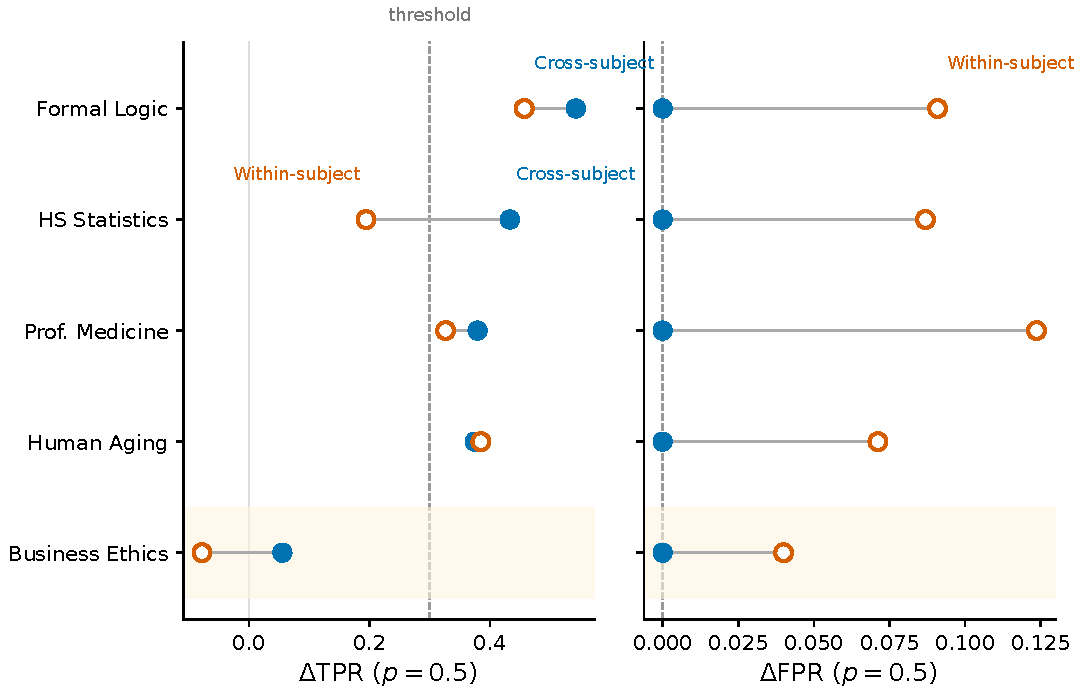
\includegraphics[width=\columnwidth]{fig_3_within_subject_matching.pdf}
\caption{Cross-subject vs.\ within-subject matching for semi-synthetic DIF detection. Cross-subject matching eliminates FPR inflation ($\Delta\mathrm{FPR} = 0.000$) while preserving detection power ($\Delta\mathrm{TPR} > 0.3$ for 4/5 subjects at $p = 0.5$). Within-subject matching inflates FPR by ${+}0.186$ on average.}
\label{fig:within_subject}
\end{figure}

\subsection{Downstream Impact}
\label{sec:downstream}

The practical relevance of 31\% item instability depends on whether unstable items affect model evaluation and benchmark rankings. We investigate this through a four-layer analysis that progresses from aggregate statistics to model-specific diagnostics.

\paragraph{Layer 1: Benchmark redundancy.} Spearman correlation between model rankings computed on all 12,508 items versus stable-only items (ETS~A/B) is $\rho \approx 0.997$. At the level of aggregate rankings, removing 31\% of items changes almost nothing. This redundancy is a consequence of the large item pool: 12,508 items provide sufficient statistical mass that removing nearly a third does not alter rank order.

\paragraph{Layer 2: Signal concentration with circularity check.} Despite aggregate redundancy, DIF-flagged items carry more discriminative signal than the average item. Removing DIF items degrades ranking discriminability more than removing an equal number of random items ($z = -8$ to $-49$ across 21 experimental conditions). A circularity ablation, however, places this in context: DIF-based removal is the \emph{least} disruptive among non-random removal strategies. Accuracy-gap removal produces $z = -156.5$, high-variance removal $z = -107.9$, and high-discrimination removal $z = -15.8$, compared to $z = -9.5$ for DIF removal. The Jaccard overlap between DIF-flagged and high-discrimination items is only 0.12. DIF items carry more signal than average, but DIF isolates differential behavior across cohorts specifically, not generally informative items.

\paragraph{Layer 3: Diagnostic lens.} Individual model families show distinctive DIF profiles that reveal which families disproportionately benefit from unstable items. Phi-3 and Llama-3 models gain ${+}700$ to ${+}850$ rank positions when evaluated on stable items only, suggesting inflated performance on items whose function changed between 2023 and 2024. Mistral-based model merges show the opposite pattern, losing $-400$ to $-587$ positions. A caveat applies: among the top 50 rank movers, most lack documented training details in METABENCH, limiting interpretation of what training choices drive these rank shifts.

\paragraph{Layer 4: Cross-benchmark signal.} The DIF instability pattern extends beyond MMLU. \Cref{sec:gsm8k} presents a full replication on GSM8K with independent contamination validation using the GSM1K held-out set~\citep{zhang2024gsm1k}. \Cref{fig:downstream} visualizes the relationship between full and DIF-filtered rankings.

\begin{figure}[t]
\centering
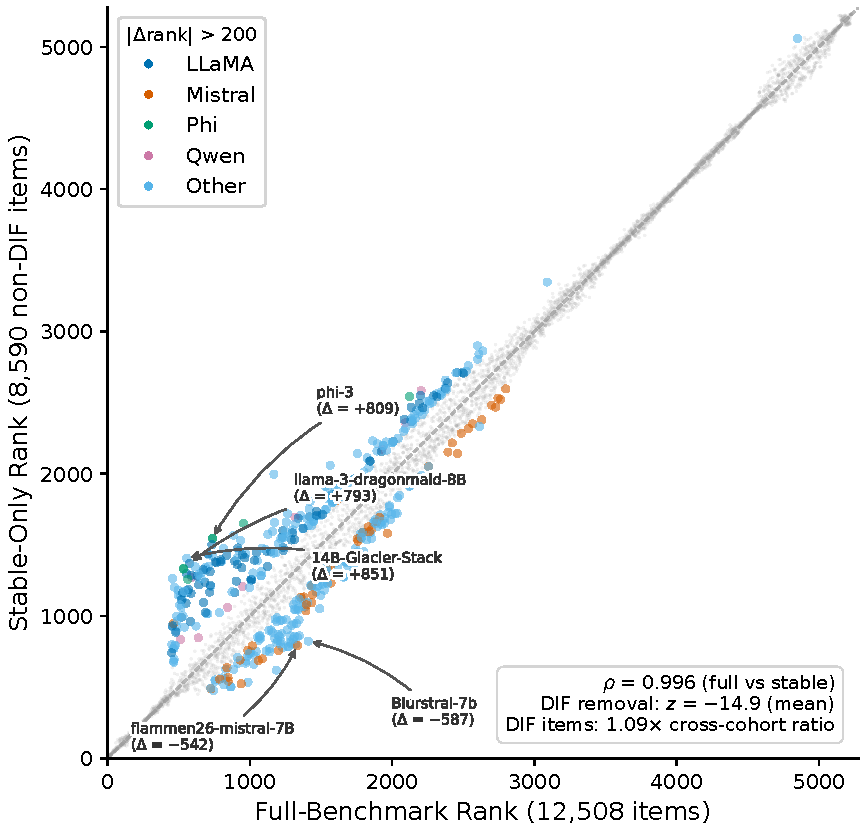
\includegraphics[width=\columnwidth]{fig_4_downstream_impact.pdf}
\caption{Downstream impact of DIF-based item filtering on model rankings. Despite $\rho \approx 0.997$ overall, individual model families show systematic rank shifts when evaluated on stable items only, with Phi-3 and Llama-3 gaining and Mistral merges losing rank positions.}
\label{fig:downstream}
\end{figure}

\subsection{Cross-Benchmark Validation: GSM8K}
\label{sec:gsm8k}

To test whether temporal DIF is specific to MMLU or reflects a broader phenomenon in LLM benchmarking, we replicate the full analysis pipeline on GSM8K (1,319 items $\times$ 6,702 models from METABENCH).

\paragraph{Temporal DIF.} Standard matching yields C\% $= 18.9\%$ for the temporal cohort comparison, with a random-split sanity check at 0.3\%. The lower instability rate compared to MMLU (31.3\%) is consistent with GSM8K's more homogeneous item structure: single-domain mathematical reasoning versus MMLU's 57 diverse subjects. The sanity check confirms that the signal is non-random.

\paragraph{Semi-synthetic validation.} Dose-response confirms detection power on this benchmark. Standard matching achieves $\Delta\mathrm{TPR} = {+}0.818$ at exploitation rate $p = 0.7$. External matching (using scores on ARC, HellaSwag, TruthfulQA, and Winogrande to match models) yields $\Delta\mathrm{TPR} = {+}0.514$ at $p = 0.5$, comparable to MMLU's ${+}0.508$ at the same exploitation rate, with $\Delta\mathrm{FPR}$ well-controlled. \Cref{tab:gsm8k_comparison} compares key metrics across both benchmarks.

\paragraph{GSM1K contamination gap.} The GSM1K dataset~\citep{zhang2024gsm1k} provides an independent measure of per-model contamination by comparing performance on the original GSM8K versus a held-out set of novel problems. For $N = 33$ models with both GSM1K scores and METABENCH evaluations, we correlate each model's contamination gap (GSM8K accuracy minus GSM1K accuracy) with the ranking advantage gained from DIF-flagged items. The observed correlation is $r = -0.478$ (95\% CI $= [-0.71, -0.16]$, $p = 0.005$; item-permutation $p = 0.014$), with partial $r = -0.385$ ($p = 0.027$) after controlling for overall accuracy. Our original hypothesis predicted a \emph{positive} correlation: models benefiting more from contamination should also benefit more from DIF items. The observed \emph{negative} correlation indicates the opposite. DIF-C items resist contamination-based performance gains, and models with larger contamination gaps benefit \emph{less} from these items. This result is suggestive at $N = 33$ and warrants replication with larger model populations, but it aligns with the broader interpretation that DIF captures item-level behavioral change distinct from simple memorization of training data. \Cref{fig:gsm1k} shows the correlation scatter.

\begin{figure}[t]
\centering
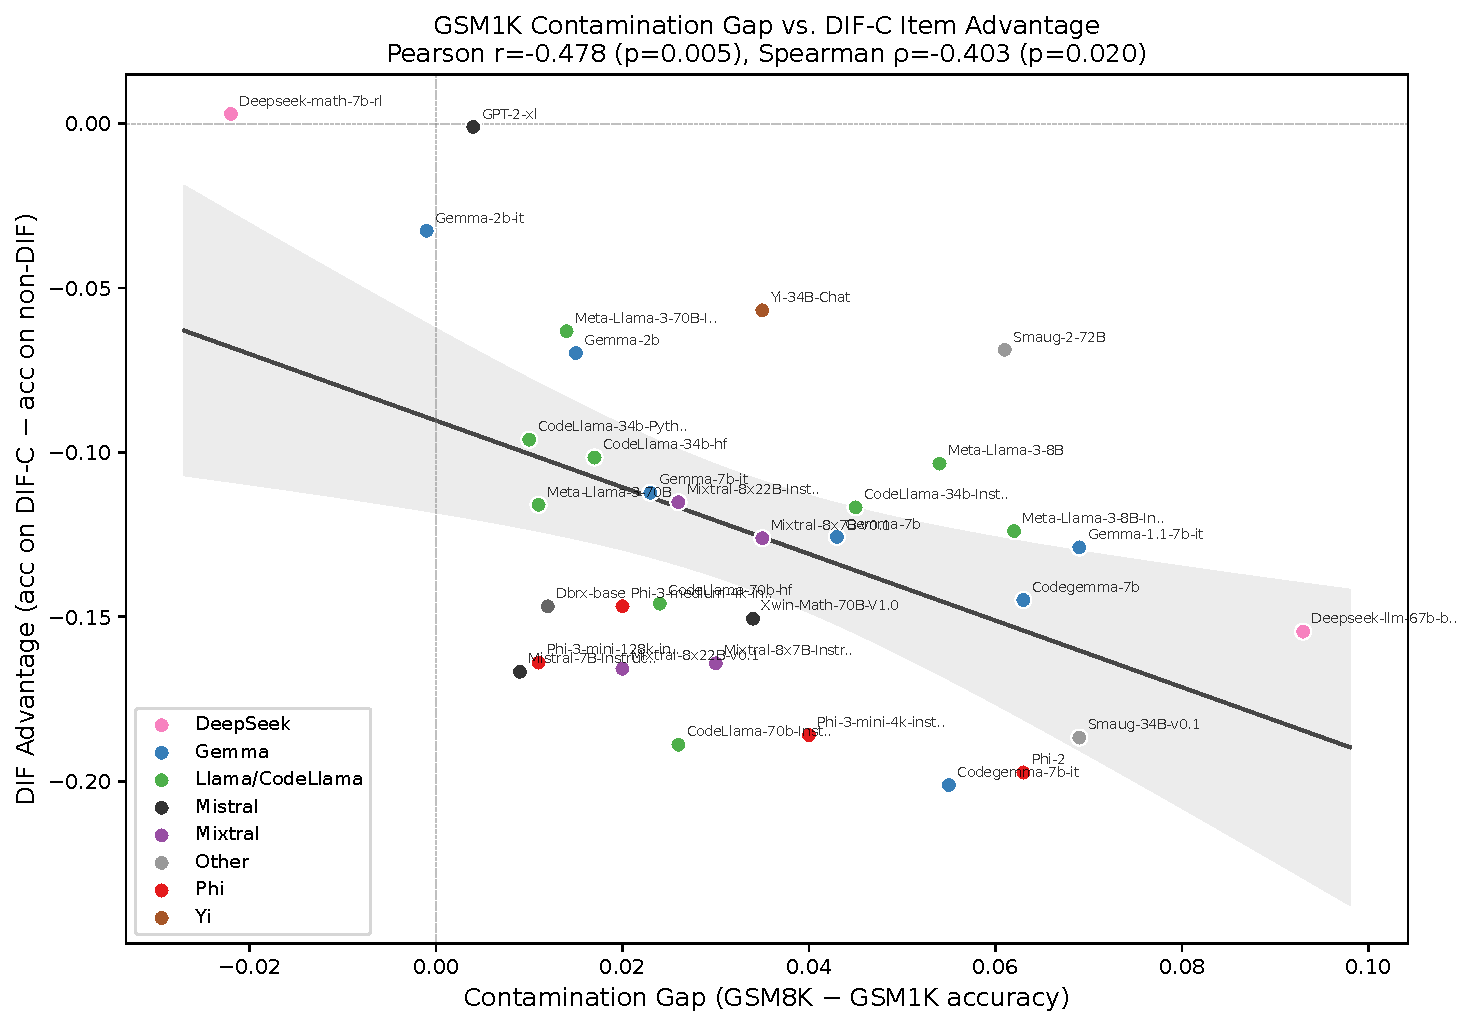
\includegraphics[width=\columnwidth]{fig_5_gsm1k_dif_correlation.pdf}
\caption{GSM1K contamination gap vs.\ DIF ranking advantage for $N = 33$ models. The negative correlation ($r = -0.478$, $p = 0.005$) indicates that models with larger contamination gaps benefit less from DIF-flagged items, contrary to the initial positive-correlation hypothesis.}
\label{fig:gsm1k}
\end{figure}

\begin{table}[t]
\centering
\caption{Cross-benchmark comparison of DIF analysis on MMLU and GSM8K. Both benchmarks exhibit temporal item instability with validated semi-synthetic detection power. Standard and external matching use different exploitation rates ($p$) because each benchmark's optimal operating point differs; external matching results are compared at $p = 0.5$ for both. Subscript $\pm$ values denote standard deviations across 5 random injection seeds.}
\label{tab:gsm8k_comparison}
\small
\begin{tabular}{lcc}
\toprule
Metric & MMLU & GSM8K \\
\midrule
Items & 12,508 & 1,319 \\
Models & 5,227 & 6,702 \\
Temporal C\% & 31.3\% & 18.9\% \\
Sanity C\% & 0.18\% & 0.3\% \\
$\Delta$TPR ($p{=}0.7$, standard) & -- & $+0.818_{\pm.006}$ \\
$\Delta$TPR ($p{=}0.5$, external) & $+0.508_{\pm.027}$ & $+0.514_{\pm.028}$ \\
\bottomrule
\end{tabular}
\end{table}

\section{Discussion}
\label{sec:discussion}
\enlargethispage*{14\baselineskip}

\subsection{Implications for Benchmark Temporal Comparability}
\label{sec:disc_temporal}

\looseness=-1
In standardized educational testing, ETS~C rates typically range from 5--15\%~\citep{clauser1998dif}; our $\approx$29\% corrected rate is 2--6$\times$ higher. Temporal DIF detects \emph{that} items function differently, not \emph{why}. Three non-exclusive mechanisms may drive this: (1)~differential contamination (asymmetric training data exposure); (2)~capability evolution (genuine skill acquisition); (3)~training methodology shifts (RLHF, post-training techniques). The difficulty--direction interaction ($\rho = -0.597$; \Cref{sec:temporal}) provides suggestive evidence for~(2): memorization would boost easy items, whereas skill acquisition disproportionately affects harder ones.

\looseness=-1
The high aggregate correlation ($\rho \approx 0.997$) does not undermine DIF's utility---MMLU's ${\sim}$12{,}500 items absorb temporal shifts at the aggregate level. DIF monitoring identifies which items shift, enabling targeted replacement and versioning~\citep{zhao2025mmlucf,habba2026growingpains}. However, this aggregate stability masks subject-level instability: mean per-subject $\rho = 0.950$, with 22/57 subjects below 0.95 and five below 0.90 (\emph{global\_facts} $0.77$, \emph{college\_mathematics} $0.82$, \emph{abstract\_algebra} $0.88$, \emph{business\_ethics} $0.89$, \emph{machine\_learning} $0.90$); smaller subjects with high C\% are disproportionately affected, making DIF monitoring critical for fine-grained comparisons.

\looseness=-1
Expert-annotated errors~\citep{gema2024mmlu} (313 items in MMLU-Redux, 4{,}802 matched) show no enrichment among DIF-C items ($0.92\times$, $\varphi = -0.01$, $p = 0.37$), confirming DIF captures dynamic shifts rather than static quality defects.

The near-independence between DIF flags and web-overlap labels (\Cref{sec:groundtruth}) reflects a category error: web-overlap measures global exposure while DIF measures differential functioning; the disconnect is in the ground truth, not detection power. MMLU-CF~\citep{zhao2025mmlucf} complements our approach: it sidesteps contamination via item reformulation, while DIF monitors which existing items are affected.

\subsection{Recommended DIF Audit Protocol}
\label{sec:disc_protocol}

\looseness=-1
Item-level properties do not reliably predict DIF susceptibility (AUROC $= 0.60$; \Cref{app:predictive}), confirming that post-hoc monitoring cannot be replaced by pre-screening.
We propose temporal MH-DIF whenever $\geq$500 models accumulate, with $\rho$-degradation-grounded action levels (\Cref{app:fig_rho_degradation}):
(1)~\emph{Monitor} (C\% $< 15\%$): report C\%.
(2)~\emph{Flag} ($15$--$25\%$): report stable-item rankings alongside full rankings.
(3)~\emph{Act} ($\geq 25\%$): prioritize flagged items for review; report stable-item rankings as primary; use DIF pre-screening for equating anchors~\citep{kolen2014equating,habba2026growingpains}.
The protocol recommends equating over removal: DIF-ordered removal degrades rankings faster than random removal (\Cref{app:fig_downstream}), confirming DIF items carry discriminating information.

\vspace{-4pt}
\section{Conclusion}
\label{sec:conclusion}

\looseness=-1
Cross-subject matching ($\Delta\mathrm{FPR} = 0.000$) resolves the validation gap (enrichment $\approx 0.96$): across six benchmarks, 17.9--31.3\% of items exhibit temporal instability (cluster bootstrap CI $[26.7\%, 53.2\%]$); benchmarks need psychometric monitoring alongside score reporting.

\section*{Limitations}

\paragraph{Methodological scope.}
MH-DIF detects only uniform DIF; logistic regression reveals an additional 24.8\% non-uniform DIF, making 31\% conservative. More fundamentally, DIF detects \emph{that} items function differently but cannot determine \emph{why}---the signal may reflect contamination, capability change, or training methodology shifts. A definitive causal decomposition remains out of reach without access to model training data.

\paragraph{Matching boundary and sample size.}
Cross-subject matching assumes contamination affects a minority of domains; when contamination spans ${>}10$ subjects (${>}18\%$ of MMLU), $\Delta\mathrm{FPR}$ rises to 0.026--0.069. The GSM1K correlation analysis ($N = 33$) has limited statistical power and is exploratory; replication with larger model samples is warranted.

\paragraph{Generalizability.}
All six benchmarks use multiple-choice or binary scoring; generalizability to open-ended generation (e.g., AlpacaEval), coding (e.g., HumanEval), or partial-credit benchmarks is untested and would require polytomous DIF methods. Temporal cohorts are defined by calendar year, a coarse grouping; finer-grained definitions (e.g., by training data cutoff or alignment method) might reveal more targeted patterns.


\bibliography{references}

\appendix
\section{Method Details}
\label{app:method_details}

\subsection{Diagnostics}
\label{app:diagnostics}

Three diagnostic procedures complement the primary DIF analysis.

\paragraph{Local independence (Yen's Q3).} The MH procedure assumes that item responses are conditionally independent given $\theta$. Yen's Q3 statistic measures residual correlations between item pairs after conditioning on the latent trait. We compute Q3 for all within-subject and cross-subject item pairs, with $|Q3| > 0.20$ as the threshold for local dependence. Elevated within-subject dependence would indicate that items within the same subject share variance beyond what $\theta$ captures, which could inflate within-subject DIF rates.

\paragraph{Domain-specificity.} We test whether temporal DIF concentrates in domains where models improved most. At the ecological level, we compute Spearman $\rho$ between subject-level C\% and subject-level accuracy improvement from 2023 to 2024. At the item level, logistic regression predicts item-level DIF~C classification from domain-level accuracy change, with and without item property controls (difficulty, discrimination). This decomposition quantifies how much of the observed instability is attributable to aggregate domain-level gains versus item-specific behavioral change.

\paragraph{Instability decomposition.} When domain accuracy improvement is included alongside item-level controls, we compute the counterfactual C\% that would remain after removing domain-level effects. The gap between observed and counterfactual C\% measures the contribution of domain-level improvement to the total instability.

\subsection{Statistical Considerations}
\label{app:statistical}

\paragraph{Multiple testing.} The ETS~C classification imposes a dual threshold (effect size $|\Delta_{\mathrm{MH}}| \geq 1.5$ and significance $p < 0.05$), which provides implicit control over false positives. As a robustness check, we apply Benjamini-Hochberg FDR correction at $q = 0.05$. The random-split sanity check provides an empirical estimate of the false positive rate under the null hypothesis.

\paragraph{Threshold sensitivity.} We report results across a range of DIF thresholds ($|\Delta_{\mathrm{MH}}| \in \{1.0, 1.5, 2.0, 2.5\}$) to verify that qualitative conclusions do not depend on the specific ETS~C cutoff. The standard threshold of $|\Delta_{\mathrm{MH}}| \geq 1.5$ corresponds to the ETS~C definition used throughout the paper.

\paragraph{Architecture heterogeneity.} The METABENCH MMLU population consists of 99.98\% decoder-only models (5,226 of 5,227). This near-complete architectural homogeneity eliminates architecture as a confound for DIF analysis. We verify this by excluding the single encoder-decoder model and confirming identical results.

\section{Structural Analysis Details}
\label{app:structural}

Three progressively refined approaches fail to reduce the temporal false positive rate below 31\%, revealing a structural property of the data rather than a methodological limitation. Matched-ability quintile analysis restricts comparisons to models of similar total score and yields enrichment ratios of 0.94--1.04, with temporal FPR unchanged at approximately 0.31. IRT $\theta$-conditioning with 20 ability strata achieves $r(\theta, \mathrm{total\ score}) = 0.9986$ and FPR $= 0.312$, confirming that the external total score already captures nearly all ability variance relevant to DIF computation. Within-subject DIF analysis on 5 representative subjects, intended to isolate subject-specific effects, finds mean C\% $= 38.1\%$, exceeding the 25\% threshold that would indicate viable bifactor structure. \Cref{tab:structural_comparison} summarizes these results.

The temporal FPR reflects genuine item-level instability that persists regardless of how ability is measured or conditioned. Yen's Q3 diagnostic reveals mild local dependence within subjects (11.3\% of within-subject item pairs exceed $|Q3| > 0.20$, vs.\ 2.2\% cross-subject; $5{\times}$ ratio, $p = 2.3 \times 10^{-9}$), which contributes to elevated within-subject DIF rates but is not the primary driver: the cross-subject matching protocol addresses this bias, and temporal C\% persists under external matching (full Q3 distributions in Appendix~Figure~A2).

\begin{table}[h]
\centering
\caption{Structural approaches to reducing temporal DIF. None reduces baseline FPR below 31\%, indicating that the observed instability is not an artifact of ability matching. Subscript $\pm$ values denote standard deviations across 5 injection seeds (baseline row only).}
\label{tab:structural_comparison}
\small
\begin{tabular}{lcccc}
\toprule
Approach & Mechanism & Temporal FPR & TPR ($p{=}0.5$) & Outcome \\
\midrule
Baseline (external) & Cross-benchmark total score & $0.314_{\pm.009}$ & $0.834_{\pm.027}$ & Reference \\
Matched-ability & Within-quintile temporal DIF & ${\sim}$0.31 & -- & Enrich.\ 0.94--1.04 \\
$\theta$-conditioning & $\theta$ replaces total score & 0.312 & 0.876 & $r(\theta,\mathrm{total}) {=} 0.9986$ \\
Within-subject & Per-subject DIF & -- & -- & C\% $= 38.1\%$ ($>$25\%) \\
\bottomrule
\end{tabular}
\end{table}

\section{Additional Figures}
\label{app:figures}

\begin{figure}[h]
\centering
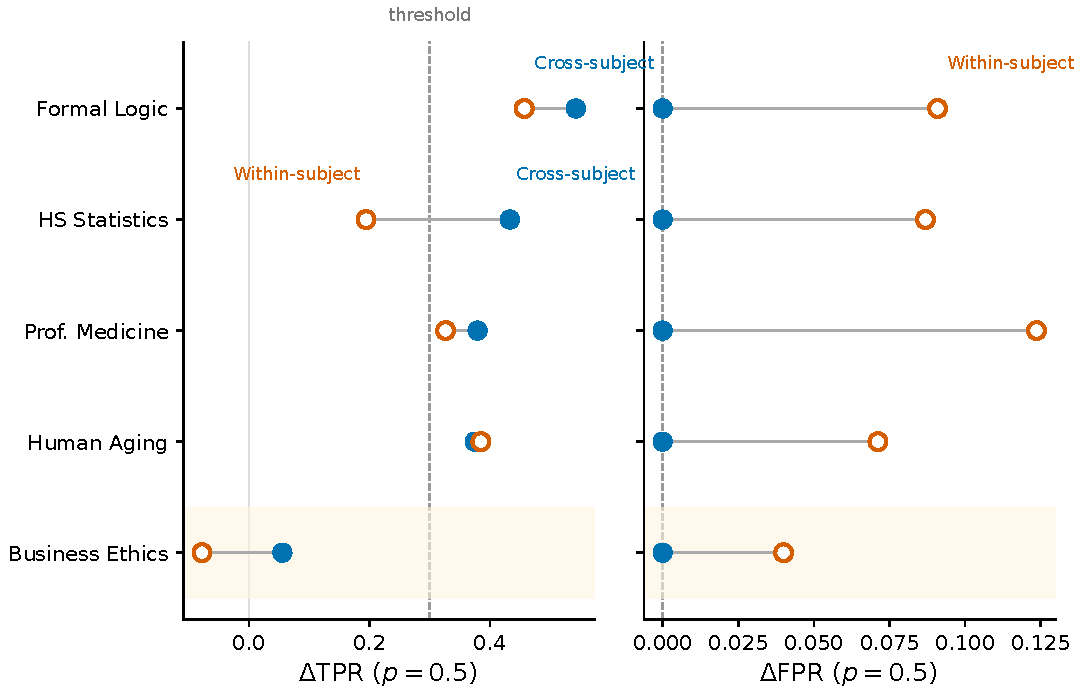
\includegraphics[width=\columnwidth]{fig_3_within_subject_matching.pdf}
\caption{Cross-subject vs.\ within-subject matching for semi-synthetic DIF detection. Cross-subject matching eliminates FPR inflation ($\Delta\mathrm{FPR} = 0.000$) while preserving detection power ($\Delta\mathrm{TPR} > 0.3$ for 4/5 subjects at $p = 0.5$). Within-subject matching inflates FPR by ${+}0.186$ on average.}
\label{app:fig_matching}
\end{figure}

\begin{figure}[h]
\centering
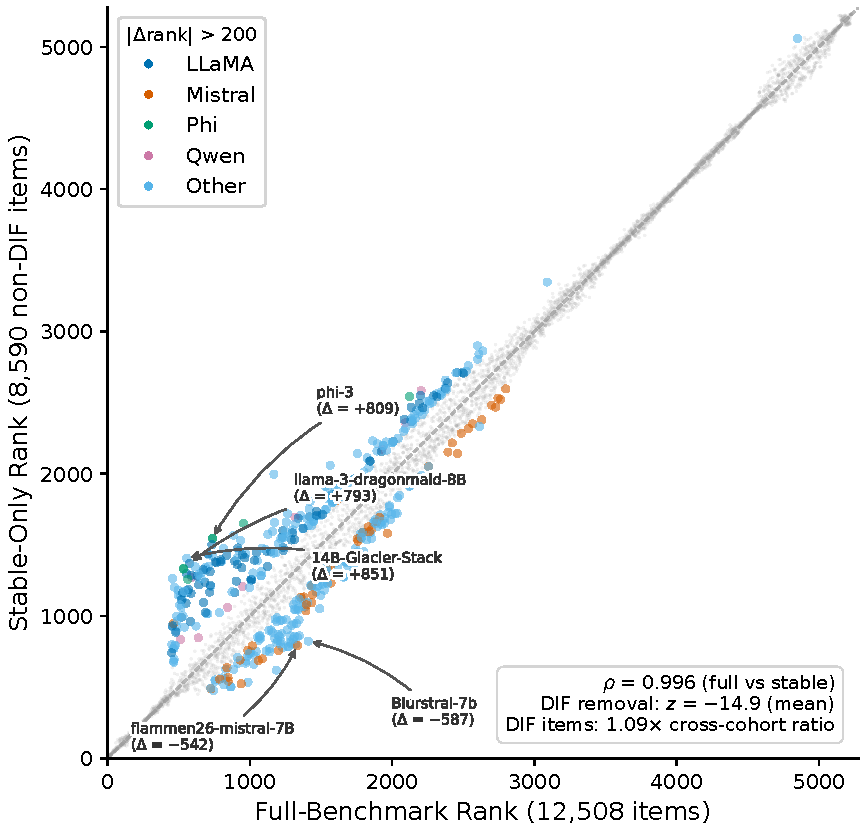
\includegraphics[width=\columnwidth]{fig_4_downstream_impact.pdf}
\caption{Downstream impact of DIF-based item filtering on model rankings. Despite $\rho \approx 0.997$ overall, individual model families show systematic rank shifts when evaluated on stable items only.}
\label{app:fig_downstream}
\end{figure}

\section{Cross-Benchmark Comparison}
\label{app:gsm8k_details}

\begin{table}[h]
\centering
\caption{Cross-benchmark comparison of DIF analysis on MMLU and GSM8K. Both benchmarks exhibit temporal item instability with validated semi-synthetic detection power. Standard and external matching use different exploitation rates ($p$) because each benchmark's optimal operating point differs; external matching results are compared at $p = 0.5$ for both. Subscript $\pm$ values denote standard deviations across 5 random injection seeds.}
\label{tab:gsm8k_comparison}
\small
\begin{tabular}{lcc}
\toprule
Metric & MMLU & GSM8K \\
\midrule
Items & 12,508 & 1,319 \\
Models & 5,227 & 6,702 \\
Temporal C\% & 31.3\% & 18.9\% \\
Sanity C\% & 0.18\% & 0.3\% \\
$\Delta$TPR ($p{=}0.7$, standard) & -- & $+0.818_{\pm.006}$ \\
$\Delta$TPR ($p{=}0.5$, external) & $+0.508_{\pm.027}$ & $+0.514_{\pm.028}$ \\
\bottomrule
\end{tabular}
\end{table}

\section{Limitations}
\label{app:limitations}

\paragraph{(a) Ecological vs.\ item-level decomposition.} The ecological correlation between subject-level C\% and accuracy improvement is $\rho = 0.307$ ($p = 0.02$), but item-level decomposition shows that domain improvement explains only 2.4 percentage points (7.6\%) of 31.3\% C\%. The remaining 92.4\% cannot be fully attributed to contamination; other sources of capability change (training methodology, data composition, optimization procedures) may contribute, and our analysis does not isolate these factors.

\paragraph{(b) Instability attribution.} The 31\% C\% measures items that function differently across cohorts, but the method does not distinguish contamination from legitimate capability change. DIF identifies \emph{that} items changed, not \emph{why}. The semi-synthetic framework validates detection power for one specific mechanism (differential exposure), but real-world instability likely reflects multiple interacting causes.

\paragraph{(c) Semi-synthetic injection fidelity.} The injection procedure flips incorrect responses to correct at a specified rate, simulating an idealized contamination scenario. Real contamination may manifest as partial knowledge, format memorization, or selective retrieval rather than wholesale answer flipping. The gap between our injection model and realistic contamination mechanisms is unknown.

\paragraph{(d) Benchmark scope.} The primary analysis covers MMLU with cross-benchmark validation on GSM8K (\Cref{sec:gsm8k}). GSM8K replication confirms framework portability and provides the GSM1K contamination correlation ($N = 33$), but full temporal DIF characterization on diverse benchmarks (code generation, long-form reasoning, multimodal tasks) has not been conducted. The GSM1K sample ($N = 33$) produces wide confidence intervals that limit the precision of the negative correlation estimate.

\paragraph{(e) Cross-subject baseline false positive rate.} The cross-subject matching protocol achieves $\Delta\mathrm{FPR} = 0.000$ for injected contamination but does not reduce the baseline temporal FPR of 33--53\% across subjects. This rate is stable across injection levels, confirming it reflects genuine temporal instability rather than methodological error, but it means that a large fraction of flagged items in temporal comparisons are not attributable to the specific contamination mechanism under test.

\paragraph{(f) RL model robustness.} Reinforcement learning from human feedback may alter item-level response patterns in ways that differ from pretraining-based contamination. The theoretical motivation for DIF robustness to RL (RL modifies the ability distribution rather than item parameters) is plausible but empirically unvalidated with adequate sample size: METABENCH contains only $N = 13$ models with documented reasoning-RL training.

\paragraph{(g) Model family coverage.} Downstream impact analysis is limited to families with $N \geq 20$ models (Llama, Mistral, Qwen, Phi). Among the top 50 rank movers, 49 of 50 belong to the ``unknown'' family category in METABENCH, precluding interpretation of what training choices produce large rank shifts.

\paragraph{(h) Future directions.} Cross-benchmark generalization to code, multimodal, and long-form reasoning benchmarks would test DIF applicability beyond factual knowledge tasks. RL model cohorts with adequate $N$ would enable empirical validation of the RL robustness hypothesis. MIMIC models and propensity-score matching could address the ability confounding that the current MH-DIF framework does not fully resolve.


\end{document}
